\chapter{Literature review}
This chapter provides an overview of past research done regarding the control of hexapod movement and of various sensing methods used. First a brief history of hexapods is presented after which various terrain sensing and adaptation methods are presented.

\section{Hexapod History}
Hexapoda, Greek for "six legs" refers the group of arthropods possessing three pairs of legs. As an example see a flesh-fly in \autoref{fig:flesh-fly}.

\begin{figure}[h]
    \centering
    \begin{minipage}{.5\textwidth}
        \centering
        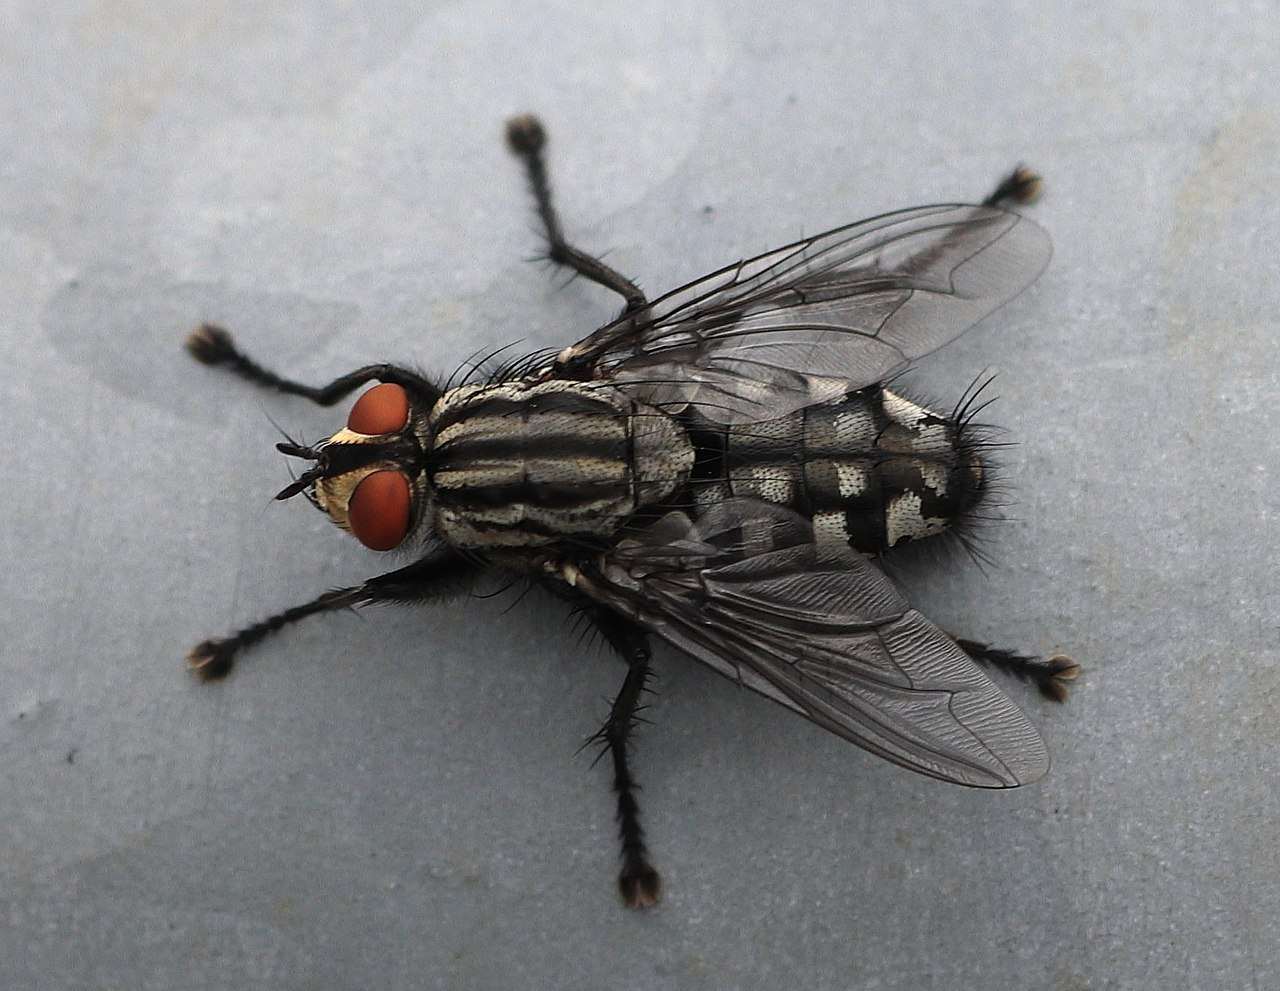
\includegraphics[height=4cm]{flesh-fly.jpg}
        \caption{A Flesh-fly}
        \label{fig:flesh-fly}
    \end{minipage}%
    \begin{minipage}{.5\textwidth}
        \centering
        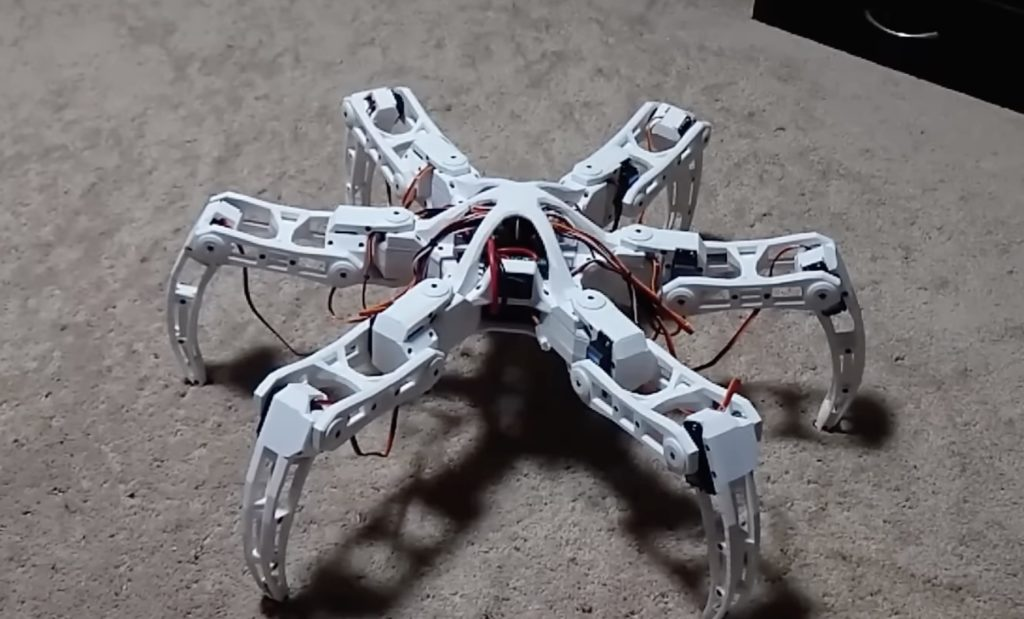
\includegraphics[height=4cm]{circ-hexapod.jpg}
        \caption{A circular hexapod}
        \label{fig:circ-hexapod}  
    \end{minipage}
\end{figure}

In the context of robotics, "hexapod" is used to refer to any robot with six legs. The most common configuration of Hexapods are either a rectangular layout with three legs on either side mimicking biological hexapoda, or a circular design with radially symmetrical leg spacing, as seen in \autoref{fig:circ-hexapod}

The hexapod possess the minimum number of legs to allow a naturally stable platform since while taking a step there can be upwards of three anchor points around the center of mass at all times. This makes the hexapod hexapods an ideal platform to navigate complex terrain while maintain stability, without requiring advanced balancing control systems.

For a hexapod to walk, it must swing some of its legs while supporting with others. The number of swinging to supporting legs, and how each is moved, is referred to as the walking "gait". The chosen gait influences the speed and stability of the hexapod. The tripod gait is considered to be the most well rounded, having good speed and stability. In the tripod gait, three legs support, while the remaining three swing. A example of a more stable gait would be the One by One gait, where only one leg is moved at a time.

It is also possible to create a system where there is no predetermined gait, but rather the system determines the optimal legs to support and swing depending on the current walking environment.

\section{Hexapod Control}
Walking over rough terrain requires a control system to correctly actuate the hexapods legs. Various types of control schemes exist. The primary schemes are traditional controllers, bio-inspired controllers and \ac{rl}. These three schemes are discussed below. Control trends can be seen in the figure below.
\begin{figure}[h]
    \centering
    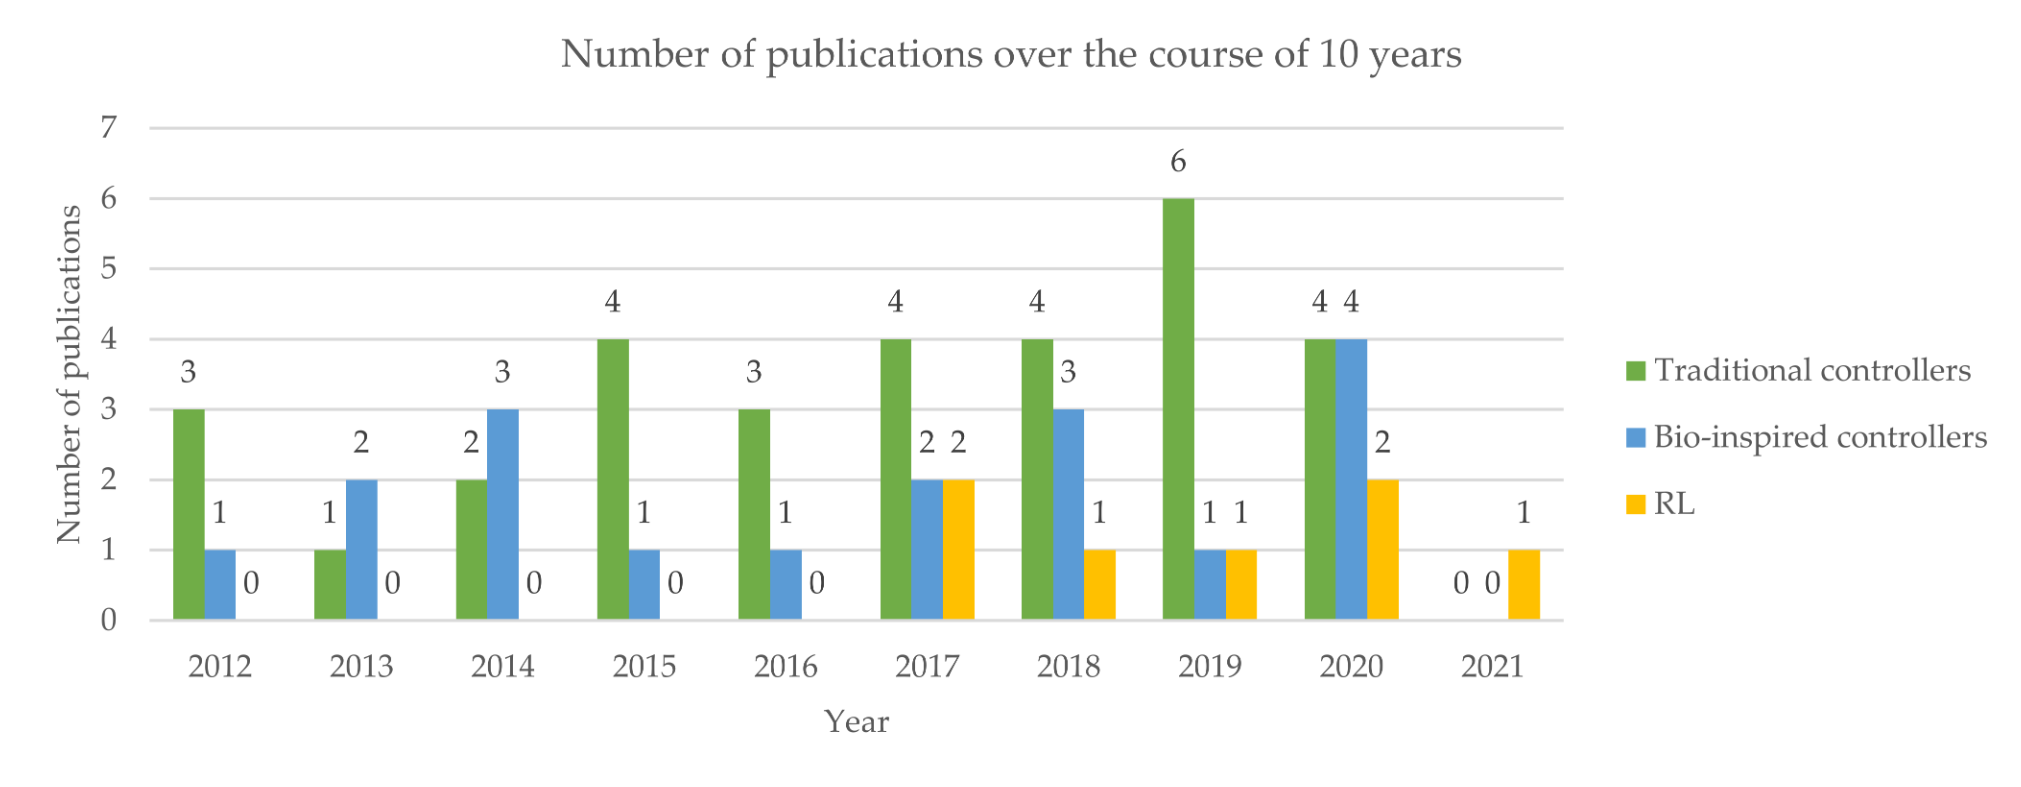
\includegraphics[width=\textwidth]{contoroller-trends.png}
    \caption{Trends of hexapod control schemes \citep{coelho2021trends}}
    \label{fig:control-trends}
\end{figure}

\noindent
As can be seen from \autoref{fig:control-trends}, traditional and bio-inspired controllers are the most widely used type of controllers, with traditional controllers being the most used. This is mostly due to the well developed theory and knowledge base that exists for traditional controllers. This makes them relatively easy to design, and they result in predictable outcomes. With the recent advancement of machine learning and neural networks, \ac{rl} control has become much more prevalent. However this technology is still quite new and can be a difficult and length process to design properly. Predicting exactly what the controller will do is also very difficult.

    \subsection{Traditional}
    Traditional controllers rely on an exact mathematical model of the robot and inverse kinematics to calculate angular commands for all leg joints. This method of control is purely kinematic and does not take into account external forces applied to the robot, thus it does not inherently adjust to the environment. \cite{Isvara2014} used kinematic control with contact sensors to allow the walking gait to be adjusted to uneven terrain. Similarly, \cite{Irwan2012} used kinematic control with contact sensors on the robot's feet. The force reading from the contact sensors were also used to control the leg actuation to minimise impact shocks. 

    Instead of a purely kinematic model, a dynamic model can also be used. When using a dynamic model, the forces acting on the robots legs are taken into account. The forces are usually acquired through torque measurements from servos. By taking applied torque into account, dynamic model controllers will intrinsically detect a deviation when an external force is applied to the robot or its legs, and compensate appropriately. \cite{Khudher2017} used this type of control for a hexapod robot designed to aid in humanitarian demining.
    
    \subsection{Bio-Inspired}
    Bio-inspired controllers attempt to mimic the neural structure of animals to achieve the same locomotion methods that they use. In mammals, locomotion commands pass through the spinal cord to the \ac{cpg} of each leg, this causes rhythmic excitations of the muscles. In robotics, this is implemented by having a high level controller, as the brain, and a lower level \ac{ann}, as the \ac{cpg} \citep{Guo2019}. If implemented successfully a bio-inspired controller can be highly adaptable to the surrounding environment and is even able to adapt to damaged or missing legs. \cite{Yu2013} used this structure, with a \ac{cpg} network that excites six \ac{vdp} oscillators. A lower level converter was used to translate the oscillators' output into angle commands for the servos. Other types of oscillators could also be used, such as the Hopf oscillator \citep{Chen2012}, which is a simpler type of oscillator. Additionally, using spiking neurons instead of oscillators is also an option, \citep{GUTIERREZGALAN202010} did this to improve computational efficiency.

    \newpage
    \subsection{\acf{rl}}
    \acf{rl} controllers are created through using trial and error to construct a neural network that minimises a cost function for a specific goal. This theoretically allows \ac{rl} controllers to adapt to any circumstances given enough time, allowing a very high level of autonomy, as no prior direction is required. \ac{rl} controllers are notoriously difficult to train properly though, especially as the number of sensors and control outputs grow large, increasing the feature space. Additionally, even the most well-trained \ac{rl} agent still has the possibility to exhibit unexpected behaviour. \cite{Liu2019} used the Monte Carlo method to optimise the gait strategy for walking over uneven terrain. While \cite{Verma2019DeepRL} proposed a method to use a supervised learning neural network to continue operation while damaged. The system would self analyse damages, and then a gait policy would be found to work with the damages.
    
\section{Terrain Sensing}
    No matter the control scheme used, to know where to place its feet the robot requires sensors to sense its environment in some way. This could be achieved through simple sensors, such as servo torque or touch. \cite{Zha2019} used contact sensors on the hexapod's feet to detect when a foot was placed on the ground. If a leg was unable to make contact with the ground, it would use the leg like a insect's feelers, searching in an area until the ground was found.

    More advanced methods, such as machine vision or \ac{lidar}, are also used. \cite{homberger2017terrain} used stereoscopic vision to adjust end effector height and to classify surface materials. \cite{Mastalli2020Motion} used vision based sensors to map and classify which parts of the terrain could be safely stepped on based on its shape.

\section{Localisation}
    Depending on the terrain navigation system it might be required to localise the robot in 3D space. For this it is possible to use external sensors such as a type of beacon (RF, Reflective, Ultrasonic) or \ac{gps}. Internal sensor could also be used, such as cameras and \acp{imu} combined with a \ac{slam} system.

    Substantial work has been done regarding \ac{slam} systems. Some of the recent algorithms include ORB-SLAM3, VIORB and RGBDSLAMv2. RGBDSLAMv2 is a popular \ac{rgbd} \ac{slam} system. It uses the RANSAC algorithm to estimate translations from the extracted features. The ICP algorithm is then used to perform a pose estimation \citep{macario2022comprehensive}.
    
    \ac{viorb} is a algorithm that is based on the older ORB-SLAM algorithm \citep{mur2017orb}. Similar to ORB-SLAM, \ac{viorb} has three main threads: tracking, local mapping and loop closing. The tracking thread estimates pose, velocity and \ac{imu} biases. The loop closing thread is used to identify keyframes that have previously been observed.

    ORB-SLAM 3 is a combination of the ORB-SLAM and \ac{viorb} algorithms, it additionally maintains a sparse map, called the atlas. The atlas contains active and dormant features. The active feature map is used by the tracking thread, while the dormant feature map is used for relocalisation \citep{macario2022comprehensive}.
    

    % \subsection{End Effector Placement Method}

    % Among other research focused on hexapods, many focus on topics such as obstacle avoidance, climbing surfaces, confined surfaces and cargo transportation.
    % When focusing of terrain adaptation most often the use of sensors such as \ac{lidar}, torque, or touch are employed. Where usually the height of end effectors
    % are adjusted to the height of the terrain \cite{coelho2021trends}.

    % Some papers, such as \cite{homberger2017terrain} utilise stereoscopic vision, in addition to end effector height adjustment, also focus on surface material classifications based on which the virtual stiffness of the impedance controller is adjusted.

    % The focus of this paper will be on end effector height and planar position adaptation through real time walkability classification of the environment. 
    % While only utilising an \ac{rgbd} camera as sensor

    % \subsection{Localisation and Mapping}

    % This project requires a system that will localise the robot within its environment, as the primary sensor used is an \ac{rgbd} camera various visual \ac{slam} systems were considered. ORB-SLAM 3, a optimisation-based, sparse map \ac{slam} system was chosen to be used. ORB-SLAM 3 maintains a sparse map, an atlas, of both active and dormant features. This atlas is used to localise in the sparse map \citep{macario2022comprehensive}.

    % The implementation of a dense map to be used for end effector placement is discussed in \autoref{chap:mapping}.


\section{Motion Over Uneven Terrain}
    As hexapods are inherently stable, they are good candidates for use in uneven terrain, and this tends to be where much hexapod research is focused.
    Such as in \cite{homberger2017terrain}, which uses a stereoscopic camera to extract features and classify terrain by factors such as material type,
    slope and granularity. These parameters are then used to classify various gait parameters, such as step height and dampening, to improve stability while
    walking.

    This is similar to \cite{Xu2023Learning}, which aims to
    classify terrain based on material properties, however, \cite{Xu2023Learning} focuses on characterising terrain through touch sensors instead of visual sensors.
    This is achieved through the use of machine learning.
    
    Moving away from gait optimisations and local terrain classification, \cite{Prágr2019Online} aims to characterize
    large areas of terrain in terms of navigational efficiency through the use of gaussian processes and a incrementally constructed spatial map.
    An example of this exploratory traversability classification can be seen in figure \ref{fig:cite_pragr}.

    \vspace{0.5cm}
    \begin{centering}
        \centering
        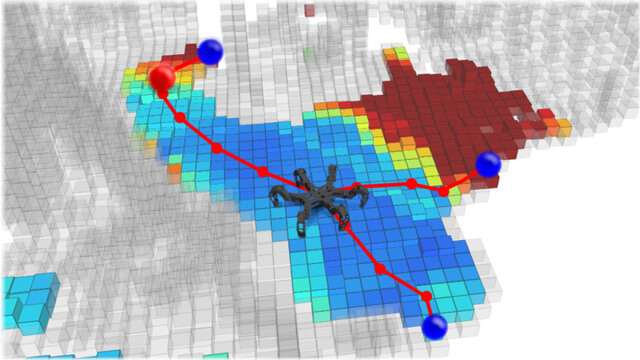
\includegraphics[width=0.7\textwidth]{cite_Pragr.jpg}
        \captionof{figure}{Exploratory terrain traversability classification from \cite{Prágr2019Online}}
        \label{fig:cite_pragr}
    \end{centering}

    \noindent
    While this paper is on hexapods, it should be noted that much work has also been done on quadrupeds. For example \cite{Mastalli2020Motion} uses various sensors
    to assign a cost to surrounding terrain, thus constructing a cost map, this cost map is then used to select optimal foot end positions for the next step. This can be seen in figure \ref{fig:cite_quadruped_walk}.
    \begin{figure}[h]
        \centering
        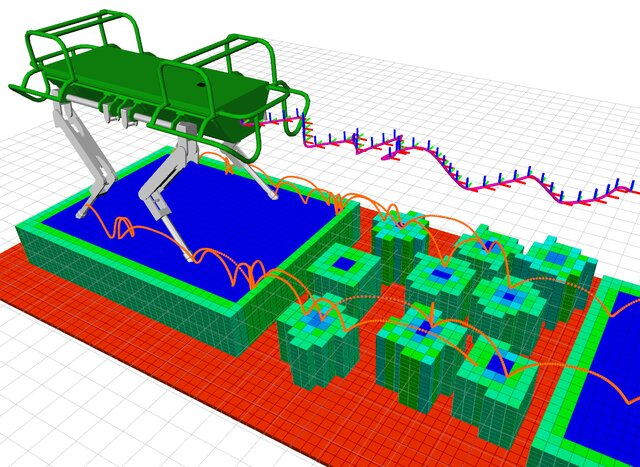
\includegraphics[width=0.8\textwidth]{cite_quadruped_score_map.jpg}
        \caption{Quadruped terrain scoring and navigation from \cite{Mastalli2020Motion}}
        \label{fig:cite_quadruped_walk}
    \end{figure}
    Of course, being a quadruped, in addition to finding optimal foot end positions, significant consideration had to be given to maintaining the stability of the robot,
    something that is much less of a concern with hexapods.

\section{Simulation Environment} \label{sec:sim_research}

The most popular physics simulators for robotics in recent times are Gazebo, \ac{mujoco},  and CoppeliaSim (previously V-REP) \citep{Collins-2021}. Gazebo and CoppeliaSim both have easy to use \ac{gui} interfaces and easy integration with \ac{ros}. \ac{mujoco} on the other hand does not have a full \ac{gui} interface, only a simulation viewer, and does not have native \ac{ros} integration. Having said this, \ac{mujoco} was found to be the most accurate and fastest simulator when considering the use case of robotics \citep{Erez-2015}.
    

\section{Research Decisions}
    Since this project focuses on using vision-based mapping, terrain classification and the optimisation of foot end positions, it was decided that traditional kinematic control will be used, as it is the simplest and most predictable method of control. This allows the focus to remain on terrain classification and foot placement optimisation.

    The camera that will be used is the Intel Realsense D435i \ac{rgbd} camera, incorporating stereoscopic cameras and a \ac{lidar} sensor. This camera also has a extensive existing codebase and support that ensures accurate depth readings are attained.

    A system to localise the robot within its environment is required. As the primary sensor used is an \ac{rgbd} camera, various visual \ac{slam} systems were considered. ORB-SLAM 3 is a relatively modern \ac{slam} algorithm that incorporates many past \ac{slam} algorithms into its design. Thus, it was decided to use ORB-SLAM3.

    Finally, a simulation environment was chosen. \ac{mujoco} has exceptional contact physics simulation and the only relevant disadvantages are its lack of native \ac{ros} integration and its lack of a comprehensive \ac{gui}. However, seeing as \ac{mujoco} has good python bindings this could be seen as a advantage. MuJuCo was therefore chosen as the simulation environment.